\documentclass[a4paper, 12pt, twoside]{article}


%------------------------------------------------------------------------
%
% Author                :   Lasercata
% Last modification     :   2022.02.06
%
%------------------------------------------------------------------------


%------ini
\usepackage[utf8]{inputenc}
\usepackage[T1]{fontenc}
\usepackage[french]{babel}
%\usepackage[english]{babel}


%------geometry
\usepackage[textheight=700pt, textwidth=500pt]{geometry}


%------color
\usepackage{xcolor}
\definecolor{ff4500}{HTML}{ff4500}
\definecolor{00f}{HTML}{0000ff}
\definecolor{0ff}{HTML}{00ffff}
\definecolor{656565}{HTML}{656565}

\renewcommand{\emph}{\textcolor{ff4500}}
\renewcommand{\em}{\color{ff4500}}

\newcommand{\strong}[1]{\textcolor{ff4500}{\bf #1}}
\newcommand{\st}{\color{ff4500}\bf}


%------Code highlighting
\usepackage{listings}

\definecolor{cbg}{HTML}{272822}
\definecolor{cfg}{HTML}{ececec}
\definecolor{ccomment}{HTML}{686c58}
\definecolor{ckw}{HTML}{f92672}
\definecolor{cstring}{HTML}{e6db72}
\definecolor{cstringlight}{HTML}{98980f}
\definecolor{lightwhite}{HTML}{fafafa}

\lstdefinestyle{DarkCodeStyle}{
    backgroundcolor=\color{cbg},
    commentstyle=\itshape\color{ccomment},
    keywordstyle=\color{ckw},
    numberstyle=\tiny\color{cbg},
    stringstyle=\color{cstring},
    basicstyle=\ttfamily\footnotesize\color{cfg},
    breakatwhitespace=false,
    breaklines=true,
    captionpos=b,
    keepspaces=true,
    numbers=left,
    numbersep=5pt,
    showspaces=false,
    showstringspaces=false,
    showtabs=false,
    tabsize=4,
    xleftmargin=\leftskip
}

\lstdefinestyle{LightCodeStyle}{
    backgroundcolor=\color{lightwhite},
    commentstyle=\itshape\color{ccomment},
    keywordstyle=\color{ckw},
    numberstyle=\tiny\color{cbg},
    stringstyle=\color{cstringlight},
    basicstyle=\ttfamily\footnotesize\color{cbg},
    breakatwhitespace=false,
    breaklines=true,
    captionpos=b,
    keepspaces=true,
    numbers=left,
    numbersep=10pt,
    showspaces=false,
    showstringspaces=false,
    showtabs=false,
    tabsize=4,
    frame=L,
    xleftmargin=\leftskip
}

%\lstset{style=DarkCodeStyle}
\lstset{style=LightCodeStyle}

%Usage : \begin{lstlisting}[language=Caml] ... \end{lstlisting}


%-------make the table of content clickable
\usepackage{hyperref}
\hypersetup{
    colorlinks,
    citecolor=black,
    filecolor=black,
    linkcolor=black,
    urlcolor=black
}


%------pictures
\usepackage{graphicx}
%\usepackage{wrapfig}

\usepackage{tikz}


%------tabular
%\usepackage{color}
%\usepackage{colortbl}
%\usepackage{multirow}


%------Physics
%---Packages
%\usepackage[version=4]{mhchem} %$\ce{NO4^2-}$

%---Commands
\newcommand{\link}[2]{\mathrm{#1} \! - \! \mathrm{#2}}
\newcommand{\pt}[1]{\cdot 10^{#1}} % Power of ten
\newcommand{\dt}[2][t]{\dfrac{d#2}{d#1}} % Derivative


%------math
%---Packages
%\usepackage{textcomp}
%\usepackage{amsmath}
\usepackage{amssymb}
\usepackage{mathtools} % For abs
\usepackage{stmaryrd} %for \llbracket and \rrbracket
\usepackage{mathrsfs} %for \mathscr{x} (different from \mathcal{x})

%---Commands
%-Sets
\newcommand{\N}{\mathbb{N}} %set N
\newcommand{\Z}{\mathbb{Z}} %set Z
\newcommand{\R}{\mathbb{R}} %set R
\newcommand{\C}{\mathbb{C}} %set C
\newcommand{\U}{\mathbb{U}} %set U
\newcommand{\set}[2]{\left[ #1\ ;\ #2 \right]}
\newcommand{\nset}[2]{\left\llbracket #1\ ;\ #2 \right\rrbracket}

%-Exponantial / complexs
\newcommand{\e}[1]{\mathrm{e}^{#1}}
\newcommand{\ex}{\e{x}}
\newcommand{\cj}[1]{\overline{#1}} %overline for the conjugate.

%-Vectors
\newcommand{\vect}{\overrightarrow}
\newcommand{\veco}[3]{\displaystyle \vect{#1}\binom{#2}{#3}} %vector + coord

%-Limits
\newcommand{\lm}[2][{}]{\lim\limits_{\substack{#2 \\ #1}}} %$\lm{x \to a} f$ or $\lm[x < a]{x \to a} f$
\newcommand{\Lm}[3][{}]{\lm[#1]{#2} \left( #3 \right)} %$\Lm{x \to a}{f}$ or $\Lm[x < a]{x \to a}{f}$
\newcommand{\tendsto}[1]{\xrightarrow[#1]{}}

%-Integral
\newcommand{\dint}[4][x]{\displaystyle \int_{#2}^{#3} #4 \mathrm{d} #1} %$\dint{a}{b}{f(x)}$ or $\dint[t]{a}{b}{f(t)}$

%-Others
\newcommand{\para}{\ /\!/\ } %//
\newcommand{\ssi}{\ \Leftrightarrow \ }
\newcommand{\abs}[1]{\left\lvert #1 \right\rvert} % abs{x} -> |x|
\newcommand{\eqsys}[2]{\begin{cases} #1 \\ #2 \end{cases}}

\newcommand{\med}[2]{\mathrm{med} \left[ #1\ ;\ #2 \right]}  %$\med{A}{B} -> med[A ; B]$
\newcommand{\Circ}[2]{\mathscr{C}_{#1, #2}}

\newcommand{\lr}[1]{\left( #1 \right)}
\newcommand{\lrb}[1]{\left[ #1 \right]}

\newcommand{\lrangle}[1]{\left\langle #1 \right\rangle}

\renewcommand{\le}{\leqslant}
\renewcommand{\ge}{\geqslant}


%------commands
%---to quote french text
\newcommand{\simplecit}[1]{\guillemotleft$\;$#1$\;$\guillemotright}
\newcommand{\cit}[1]{\simplecit{\textcolor{656565}{#1}}}
\newcommand{\quo}[1]{\cit{\it #1}}

%---to indent
\newcommand{\ind}[1][20pt]{\advance\leftskip + #1}
\newcommand{\deind}[1][20pt]{\advance\leftskip - #1}

%---to indent a text
\newcommand{\indented}[2][20pt]{\par \ind[#1] #2 \par \deind[#1]}
\newenvironment{indentedenv}[1][20pt]{\par \ind[#1]}{\par \deind}
\newenvironment{indt}[2][20pt]{#2 \begin{indentedenv}[#1]}{\end{indentedenv}} %Titled indented env

%---title
\newcommand{\thetitle}[2]{\begin{center}\textbf{{\LARGE \underline{\emph{#1} :}} {\Large #2}}\end{center}}

%---parts
%-I
\newcommand{\mainpart}[2][$\!\!$]{\underline{\large \textbf{\emph{\textit{#1} #2}}}}
\newcommand{\bmainpart}[2][$\!\!$]{\underline{\large \textbf{\textit{#1} #2}}}
%-A
\newcommand{\subpart}[2][$\!\!$]{\underline{\bf \textit{#1} #2}}
%-1
\newcommand{\subsubpart}[2][$\!\!$]{\underline{\textsl{#1} #2}}
%-a
\newcommand{\subsubsubpart}[2][$\!\!$]{\underline{\it #1 #2}}

%math part
\newcommand{\secpart}[1]{.\underline{\it #1 :}}

\newenvironment{mathdef}[2][20pt]{
    \secpart{#2} \begin{indentedenv}[#1]}
    {\end{indentedenv}}


%------page style
\usepackage{fancyhdr}
\usepackage{lastpage}

\setlength{\headheight}{18pt}
\setlength{\footskip}{50pt}

\pagestyle{fancy}
\fancyhf{}
\fancyhead[LE, RO]{\textit{\today}}
\fancyhead[RE, LO]{\large{\textsl{\emph{\texttt{\jobname}}}}}

\fancyfoot[RO, LE]{\textit{\texttt{Page \thepage /\pageref{LastPage}}}}
\fancyfoot[LO, RE]{\includegraphics[scale=0.12]{/home/lasercata/Pictures/1.images_profil/logo/mieux/lasercata_logo_fly_fond_blanc.png}}


%------init lengths
\setlength{\parindent}{0pt} %no \noindent needed !!!
\setlength{\parskip}{3pt}


%---------------------------------Begin Document
\begin{document}

    \thetitle{Chapitre 3}{Vérification de programme}
    
    \tableofcontents
    
    \newpage
    
    
    \begin{indt}{\section{Terminaison}}
        
        \begin{indt}{\subsection{Définition (terminaison)}}
            On dit qu'un programme / algorithme termine s'il n'éxécute qu'un nombre fini d'opérations quelle que soit l'entrée.
        \end{indt}
        
        \begin{indt}{\subsection{Remarque}}
            Le nombre d'opérations peut être arbitrairement grand en fonction de l'entrée (pas de majorant commun à toutes les entrées).
            
            Si $\exists c \ |\ \forall n,\ C(n) \le c \ \longrightarrow O(1)$
        \end{indt}
        
        \begin{indt}{\subsection{Exemple}}
            Montrons que les deux fonctions suivantes terminent :
            
            \begin{lstlisting}[language=Caml, xleftmargin=60pt]
let is_prime (n : int) : bool =
    let res = ref true in
    for i = 2 to n - 1 do
        if n mod i = 0 then
            res := false
    done;
    !res\end{lstlisting}
            
            \vspace{6pt}
            
            La boucle est éxécutée $n - 2$ fois, et contient uniquement des opérations élémentaires qui terminent.
            
            \vspace{6pt}
            
            \begin{lstlisting}[language=Caml, xleftmargin=60pt]
let count_primes (n : int) : int =
    let res = ref 0 in
    for i = 2 to n do
        if is_prime i then incr res
    done;
    !res\end{lstlisting}
            
            \vspace{6pt}
            
            La boucle est éxécutée $n - 1$ fois, chaque appel à \texttt{is\_prime} termine, et le reste est composé d'opérations élémentaires qui terminent.
            
            \vspace{6pt}
            
            Conclusion : une boucle inconditionnelle termine dès que les opérations qui le composent terminent.
            
            \vspace{6pt}
            
            Attention : une boucle \texttt{for} en C est une boucle \texttt{while} déguisée.
            
            Rappel
            
            \begin{lstlisting}[language=C, xleftmargin=60pt]
for (c1 ; c2 ; c3) c4
//Is equivalent to
{
    c1;
    while (c2) {
        c4;
        c3;
    }
}\end{lstlisting}
            
            \vspace{6pt}
            
            La difficulté dans les preuves de terminaison réside dans les boucles \texttt{while} et les fonctions récursives.
        \end{indt}
        
        \vspace{6pt}
        
        \begin{indt}{\subsection{Définition (variant)}}
            Un variant est une quantité entière positive au début de chaque itération / appel récursif et telle que sa valeur décroît strictement au cours de l'itération.
            
            Généralisation : on peut autoriser les quantités négatives strictement croissantes.
        \end{indt}
        
        \vspace{6pt}
        
        \begin{indt}{\subsection{Théorème}}
            Une boucle composée d'opérations qui terminent et admettant un variant termine.
            
            $\square$ Il n'existe pas de suite strictement décroissante d'entiers positifs. $\blacksquare$
            
            $\nexists (u_n) \in \N^\N \ |\ \forall n \in \N,\ u_{n + 1} < u_n$
            
            $\forall (u_n) \in \N^\N,\ \exists n \in \N\ |\ u_{n + 1} \ge u_n$.
        \end{indt}
        
        \vspace{6pt}
        
        \begin{indt}{\subsection{Exemple}}
            \begin{lstlisting}[language=C, xleftmargin=60pt]
while (a > 0 && b > 0) {
    if (a % 2 == 0) {
        a++;
        b -= 3;
    }
    else {
        a -= 2;
        b++;
    }
}\end{lstlisting}
            
            $\bullet$ Si $a \le 0$ ou $b \le 0$, on n'entre pas dans la boucle.
            
            \begin{indt}{$\bullet$ Si $a > 0$ et $b > 0$,}
            $-$ \texttt a est un variant à partir de la deuxième itération (\texttt a pair $\rightarrow$ \texttt{a + 1} impair puis des soustractions avec 2 conservent la parité)
            
            $-$ \texttt{a + b} est un variant.
            \end{indt}
        \end{indt}
        
        \vspace{6pt}
        
        \begin{indt}{\subsection{Cas des fonctions récursives}}
            \begin{lstlisting}[language=Caml, xleftmargin=60pt]
let rec is_even (n : int) : bool =
    match n with
    | 0 -> true
 (* | 1 -> false *)
    | _ -> is_even (n - 2)\end{lstlisting}
            
            Le variant "naturel" ($n$) peut devenir négatif si on oublie un cas d'arrêt.
            
            Trouver une quantité strictement décroissante ne suffit pas, il faut vérifier que l'on atteint toujours un cas d'arrêt.
            
            \vspace{6pt}
            
            En cas de doute, on peut toujours écrire une fonction récursive comme une boucle \texttt{while}.
            
            On parle de dérécursivation (H.P. dans sa généralité), simple dans le cas des fonctions récursives terminales.
            
            \begin{lstlisting}[language=Caml, xleftmargin=60pt]
let is_even (n : int) : bool =
    let m = ref n in
    while !m <> 0 && !m <> 1 do
        m := !m - 2
    done;
    !m = 0
            \end{lstlisting}
        \end{indt}
        
    \end{indt}
    
    \vspace{12pt}
    
    \begin{indt}{\section{Correction}}
        
        \begin{indt}{\subsection{Définition (correction)}}
            On dit qu'un algorithme / programme est correct vis-à-vis d'une spécification si, quelle que soit l'entrée, il termine et renvoit un résultat qui respecte la spécification.
            
            \vspace{6pt}
            
            On parle de \textit{correction totale} par contraste avec la \textit{correction partielle}, définie comme suit :
            
            Un programme / algorithme est \textit{partiellement} correct vis-à-vis d'une spécification si, quelle que soit l'entrée \textit{telle que le programme termine}, le résultat renvoyé respecte la spécification.
        \end{indt}
        
        \vspace{6pt}
        
        \begin{indt}{\subsection{Exemple}}
            \begin{lstlisting}[language=Caml, xleftmargin=60pt]
let rec sum (n : int) : int =
    if n = 0 then 0
    else n + sum (n - 1)\end{lstlisting}
            
            Partiellement correct
            
            \begin{lstlisting}[language=Caml, xleftmargin=60pt]
let rec sum (n : int) : int =
    assert (n >= 0);
    if n = 0 then 0
    else n + sum (n - 1)\end{lstlisting}
            
            Spécification : $\forall n \in \Z$, \texttt{sum} vaut $\displaystyle \sum_{k = 0}^n k$.
            
            Termine bien dans tous les cas, mais ne renvoit pas de résultat dans le cas $n < 0$.
        \end{indt}
        
        \vspace{6pt}
        
        \begin{indt}{\subsection{Définition (invariant)}}
            Un invariant est un prédicat portant sur les variables du programme, qui est satisfait avant d'entrer dans la boucle / au début du premier appel (récursif) et tel que l'éxécution d'une itération conserve sa véracité.
        \end{indt}
        
        \vspace{6pt}
        
        \begin{indt}{\subsection{Remarque}}
            L'objectif est de trouver un invariant tel que sa véracité en sortie de boucle guarantit la spécification.
        \end{indt}
        
        \vspace{6pt}
        
        \begin{indt}{\subsection{Exemple}}
            \begin{lstlisting}[language=Caml, xleftmargin=60pt]
let suplog2 (n : int) : int =
    let k = ref 0 in
    let p = ref 1 in
    while !p < n do
        incr k;
        p := 2 * !p
    done;
    !k
            \end{lstlisting}
            
            Terminaison : \texttt{n - !p} est un variant.
            
            \vspace{6pt}
            
            \begin{indt}{Correction : on montre que $I(k, p) = (2^{k - 1} < n\ \text{et}\ p = 2^k)$ est un invariant :}
                $-$ Avant d'entrer dans la boucle, $I(0, 1) = (2^{-1} < n\ \text{et}\ 1 = 2^0)$ : ok.
                
                $-$ Si $I(k, p)$ est vrai au début d'une itération, on veut montrer $I(k + 1, 2p)$ :
                
                \vspace{6pt}
                
                $I(k + 1, 2p) = (2^k < n\ \text{et}\ 2p = 2^{k + 1})$
                
                \vspace{6pt}
                
                $-$ $2^k < n$ : vrai car $2^k = p < n$ puisque la condition de boucle était vraie au début de l'itération ;
                
                $-$ $2p = 2^{k + 1}$ : vrai car $p = 2^k$ d'après $I(k, p)$.
            \end{indt}
            
            \vspace{6pt}
            
            $I$ en sortie de boucle démontre la correction : on a $I(k, p) = (2^{k -1} < n\ \text{et}\ p = 2^k)$ et la condition de boucle est fausse, \textit{i.e} $p \ge n$ donc $2^k \ge n$. %$2^{k - 1} \le 2^k$
            
            \vspace{12pt}
            
            Attention, cette démonstration est fausse !
            
            Ex : $n = \underbrace{\lrangle{0111\ldots1}_2}_{\text{nombre de bits du type \texttt{int}}}$ (type d'entiers signés)
            
            $p : \lrangle{0\ldots01}_2$ puis $\lrangle{0\ldots010}_2$ puis $\ldots$ puis $\lrangle{01\ldots0}_2 < n$
            
            Or si $p = \lrangle{01\ldots0}_2$, alors $2p < 0 < n$
            
            \vspace{6pt}
            
            Il peut y avoir des dépassement de capacité : il faut en tenir compte dans la spécification, ou bien détecter l'\textit{overflow} dans le calcul.
        \end{indt}
        
        %\vspace{6pt}
        
        \begin{indt}{\subsection{Exercice : suite de Fibonacci}}
            \begin{lstlisting}[language=C, xleftmargin=60pt]
int fibo(int n) {
    int x = 1, y = 1;
    for (int i = 0 ; i < n - 1 ; i++) {
        y = x + y;
        x = y - x;
    }
    return y;
}\end{lstlisting}
            
            On note $(F_n)_{n \in \N}$ les termes de la suite de Fibonacci.
            
            $I(i, x, y) = (y = F_{i + 1}\ \text{et}\ x = F_i)$
        \end{indt}
        
    \end{indt}
    
    \vspace{12pt}
    
    \begin{indt}{\section{Graphe de flot de contrôle}}
        
        \begin{indt}{\subsection{Motivation}}
            En pratique, il est difficile de trouver des invariants pour démontrer la correction d'un programme. Il est possible de démontrer des propriétés sur un programme à l'aide d'outils qui analysent le code sans l'exécuter (on parle d'analyse statique), mais ils ne permettent pas de tout démontrer : on fait en général des tests.
            
            \quo{Program testing can be used to show the presence of bugs, but never to show their absence !} Edsger W. Dÿkstra
            
            \quo{Beware of bugs in the above code ; I have only proven it correct, not tried it.} Donald E. Knuth
            (ex : compilateur bugé, ...)
            
            \vspace{12pt}
            
            Le choix des tests est particulièrement important pour ne pas ``manquer'' des erreurs.
            
            Une analyse de la structure du code peut aider à les concevoir.
        \end{indt}
        
        \vspace{12pt}
        
        \begin{indt}{\subsection{Graphe de flot de contrôle}}
            Définition : Un graphe de flot de contrôle est un graphe orienté représentant la structure d'un programme.
            Il possède un point d'entrée et un point de sortie correspondant à l'entrée et à la sortie du programme.
            Ses sommets sont de deux natures : il y a des blocs d'instructions élémentaires et des noeuds de décision étiquetés par une condition et correspondant aux branchements dans l'exécution du programme.
            Les arcs du graphe relient les noeuds correspondant à des blocs d'instructions et branchements consécutifs.
            
            \vspace{12pt}
            
            \begin{indt}{Construction :}
                $-$ Les instructions élémentaires consécutives sont réunies dans un même bloc
                
                Ex :
                \begin{tabular}{ccccc}
                    E
                    &
                    $\rightarrow$
                    &
                    \begin{lstlisting}[language=C]
int x = 1;
int y = 2;
x = x + y;
y = x - y;
x = x - y;\end{lstlisting}
                    &
                    $\rightarrow$
                    &
                    S
                \end{tabular}
                
                \vspace{12pt}
                
                $-$ Une instruction conditionnelle crée un branchement :
                \texttt{if b then c1 else c2}
                
%                 \begin{tabular}{ccccc}
%                     E
%                     & $\rightarrow$
%                     & b
%                     & $\underbrace{\rightarrow}_{\text{true}}$
%                     & \fbox{c1}
%                     \\
%                     && $\downarrow$ false
%                     && $\downarrow$
%                     \\
%                     && \fbox{c2}
%                     & $\rightarrow$
%                     & S
%                 \end{tabular}
                
                \begin{center}
                    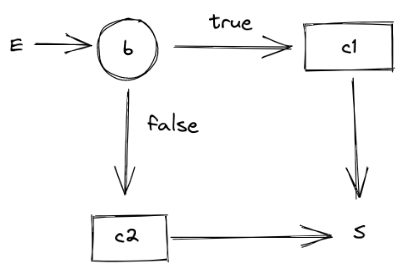
\includegraphics[scale=.3]{draw/draw0.png}
                \end{center}
                
                \vspace{12pt}
                
                $-$ Une boucle crée également un branchement :
                
                \begin{lstlisting}[language=C, xleftmargin=80pt]
while (b) {
    c
}\end{lstlisting}
                
%                 \begin{tabular}{ccccc}
%                     &&& $\leftarrow$
%                     \\
%                     && $\downarrow$
%                     && $\uparrow$
%                     \\
%                     E
%                     & $\rightarrow$
%                     & b
%                     & $\underbrace{\rightarrow}_{\text{true}}$
%                     & \fbox{c}
%                     \\
%                     && $\downarrow$ false
%                     \\
%                     && S
%                 \end{tabular}
                
                \begin{center}
                    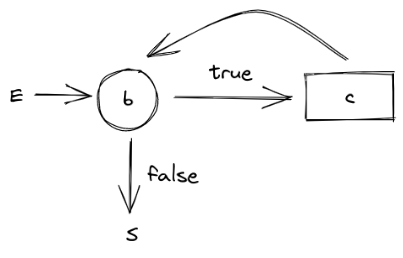
\includegraphics[scale=.4]{draw/draw_while.png}
                \end{center}
                
                \vspace{6pt}
                
                On pourra voir une boucle \texttt{for} comme une boucle \texttt{while}
                
                \begin{lstlisting}[language=C, xleftmargin=80pt]
for (c1; c2; c3)
    c4;\end{lstlisting}
                
                \begin{center}
                    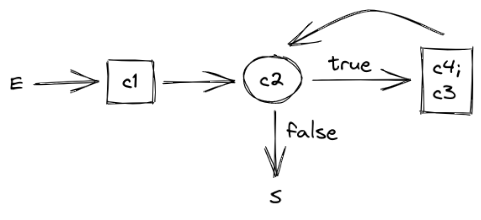
\includegraphics[scale=0.4]{draw/draw1.png}
                \end{center}
                
                On peut adopter cela en OCaml en écrivant une condition qui porte sur la variable de boucle.
                
                \begin{lstlisting}[language=Caml, xleftmargin=80pt]
for i = a to b do
    c
done\end{lstlisting}
                
%                 \fbox{
%                 \begin{tabular}{ccccccc}
%                     E
%                     & $\rightarrow$
%                     &\fbox{i $\leftarrow$ a}
%                     & $\rightarrow$
%                     & $i \le b$
%                     & $\underbrace{\rightarrow}_{\text{true}}$
%                     & \fbox{c; i $\leftarrow$ i+1}
%                     \\
%                     &&&& $\downarrow$ false
%                     \\
%                     &&&& S
%                 \end{tabular}
%                 }
                
                \begin{center}
                    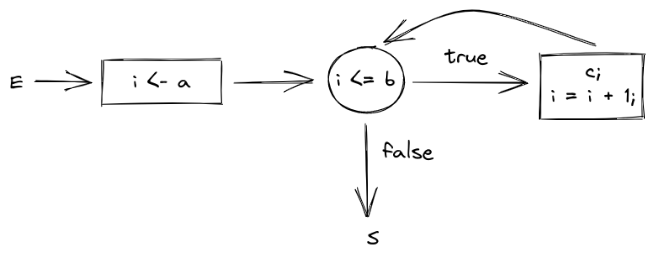
\includegraphics[scale=.4]{draw/draw_for_caml.png}
                \end{center}
                
                \vspace{12pt}
                
                Ex : calcul du PGCD par soustractions succesives
                
                \begin{lstlisting}[language=C, xleftmargin=80pt]
while (p != q) {
    if (p > q)
        p = p - q;
    
    else
        q = q - p;
}

return p;\end{lstlisting}
                \begin{center}
                    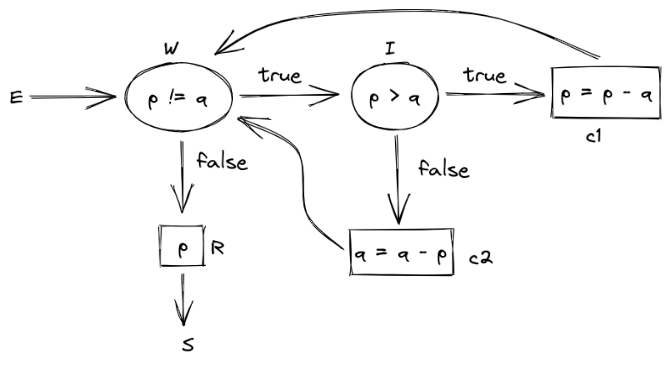
\includegraphics[scale=.37]{draw/PGCD.png}
                \end{center}
            \end{indt}
        \end{indt}
        
        \vspace{12pt}
        
        \begin{indt}{\subsection{Chemins et exécutions}}
            Une éxécution du programme correspond à un chemin dans son graphe de flot de contrôle.
            
            Ex : PGCD avec $p = 6$ et $q = 10$, on obtient le chemin
            \texttt{E $\rightarrow$ W $\rightarrow$ I $\rightarrow$ c2 $\rightarrow$ W $\rightarrow$ I $\rightarrow$ c1 $\rightarrow$ W $\rightarrow$ I $\rightarrow$ c2 $\rightarrow$ W $\rightarrow$ R $\rightarrow$ S}
            
            Un chemin ne correspond pas forcément à une exécution.
            
            Par exemple :
            
            \begin{lstlisting}[language=C, xleftmargin=60pt]
if b then x := 0;
if !x <> 0 then y := 1 / !x\end{lstlisting}
            
            \begin{center}
                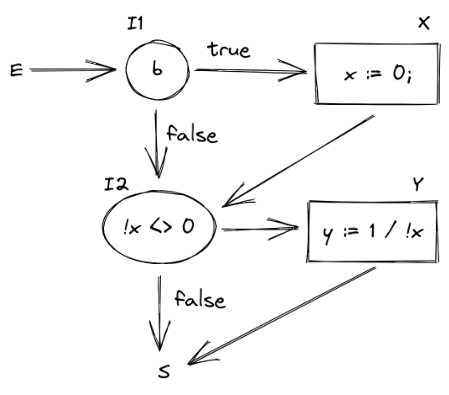
\includegraphics[scale=.4]{draw/draw2.png}
            \end{center}
            
            Le chemin \texttt{E $\rightarrow$ I1 $\rightarrow$ X $\rightarrow$ I2 $\rightarrow$ Y $\rightarrow$ S} ne correspond à aucune exécution.
            
            \vspace{12pt}
            
            On appelle chemin faisable un chemin qui correspond à (au moins) une exécution.
            
            \begin{indt}{Le principe de la conception de tests à l'aide du graphe de flots de contrôle est le suivant :}
                1) On choisit un ensemble de chemins selon un critère de couverture fixée à l'avance ;
                
                2) On élimine les chemins infaisables ;
                
                3) Pour chaque chemin restant, on étudie les conditions qui portent sur les entrées du programme pour que l'exécution correspondante au chemin. On choisit alors une entrée comme cas de test.
            \end{indt}
        \end{indt}
        
        \vspace{12pt}
        
        \begin{indt}{\subsection{Critère de couverture}}
            Pour couvrir tous les cas possibles, le critère le plus évident est de prendre tous les chemins possibles.
            
            Par exemple, pour le graphe en 3.3., on a les chemins suivants :
            
%             \begin{tabular}{ccccccccccc}
%                 E
%                 & $\rightarrow$
%                 & I1
%                 & $\rightarrow$
%                 & X
%                 & $\rightarrow$
%                 & I2
%                 & $\rightarrow$
%                 & Y
%                 & $\rightarrow$
%                 & S
%                 \\
%                 && |
%                 &&&& $\quad \searrow$
%                 \\
%                 && |
%                 &&&&& S
%                 \\
%                 && $\quad \searrow$
%                 \\
%                 &&& I2
%                 & $\rightarrow$
%                 & Y
%                 & $\rightarrow$
%                 & S
%                 \\
%                 &&& $\quad \searrow$
%                 \\
%                 &&&& S
%             \end{tabular}
            
    
            \begin{tikzpicture}[node distance = 35pt]
                \node (E) {E};
                \node (I1) [right of = E] {I$_1$};
                \node (X) [right of = I1] {X};
                \node (I2) [right of = X] {I$_2$};
                \node (Y) [right of = I2] {Y};
                \node (S) [right of = Y] {S};
                
                \node (S2) [below right of = I2] {S};
                
                \node (I22) [below of = I1] {I$_2$};
                \node (Y2) [right of = I22] {Y};
                \node (S3) [right of = Y2] {S};
                
                \node (S4) [below right of = I22] {S};
                
                
                \draw[->] (E) -- (I1);
                \draw[->] (I1) -- (X);
                \draw[->] (X) -- (I2);
                \draw[->] (I2) -- (Y);
                \draw[->] (Y) -- (S);
                
                \draw[->] (I2) -- (S2);
                
                \draw[->] (I1) -- (I22);
                \draw[->] (I22) -- (Y2);
                \draw[->] (Y2) -- (S3);
                
                \draw[->] (I22) -- (S4);
            \end{tikzpicture}
            
            \vspace{6pt}
            
            Cependant, dès qu'il y a une boucle, il y a une infinité de chemins dans le graphe.
            
            Rq : on peut avoir une infinité de chemins faisables même si le programme termine (ex : une boucle dont le nombre d'itérations dépend d'une variable d'entrée)
            
            On peut affaiblir ce critère en considérant tous les chemins de longueur au plus $k$ (fixé) ou tous les chemins qui vont parcourir la boucle au plus $k$ fois.
            
            \vspace{12pt}
            
            \begin{indt}{On peut choisir d'autres critères, comme :}
                $-$ La couverture de toutes les instructions du programme : on choisit un ensemble de chemins tels que chaque sommet est couvert par au moins un chemin.
                
                Ex :
                \begin{lstlisting}[language=C, xleftmargin=80pt]
if (x != 0)
    x = 1;
y = 1 / x;\end{lstlisting}
                
                \begin{center}
                    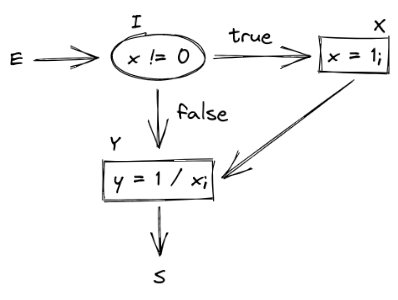
\includegraphics[scale=.4]{draw/draw3.png}
                \end{center}
                
                Le chemin \texttt{E $\rightarrow$ I $\rightarrow$ X $\rightarrow$ Y $\rightarrow$ S} satisfait le critère mais ne couvre pas la division par 0.
                
                \vspace{12pt}
                
                $-$ La couverture de toutes les branches : on choisit un ensemble de chemins tels que pour chaque noeud de décision, les deux branches issues de ce noeud sont couvertes par au moins un chemin.
                
                Ex :
                \begin{lstlisting}[language=Caml, xleftmargin=80pt]
if a < 2 && b = a then
    x := 2 - a
else
    x := a - 2\end{lstlisting}
                
                \begin{center}
                    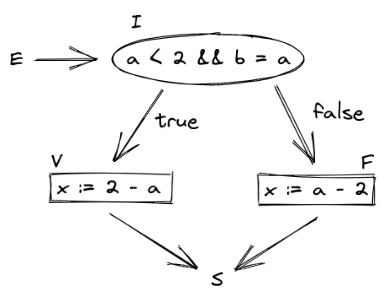
\includegraphics[scale=.4]{draw/draw4.png}
                \end{center}
                
                Le critère est satisfait par l'ensemble de chemins \{ \texttt{E $\rightarrow$ I $\rightarrow$ V $\rightarrow$ S, E $\rightarrow$ I $\rightarrow$ F $\rightarrow$ S} \}.
                
                Ces chemins sont faisables ($a = b = 1$ et $a = b = 3$)
                
                La couverture des boucles implique la couverture des instructions mais pas nécessairement la couverture de toutes les possibilités (il manque le cas où $a \neq b$)
                
                Il est possible de rajouter comme contrainte le choix des tests couvrant toutes les valeurs possibles par les sous-conditions, mais le nombre de tests devient exponnetiel en le nombre de sous-conditions.
                
                Rq : il n'est pas forcément intéressant de considérer toutes les valeurs par les sous-conditions (ex : évaluation paresseuse des opérateurs booléens)
            \end{indt}
        \end{indt}
        
        \vspace{12pt}
        
        \begin{indt}{\subsection{Détection des chemins infaisables et choix des tests}}
            \begin{indt}{Afin de déterminer si un chemin est faisable et, le cas échéant, de choisir un test concret le réalisant, on peut calculer une ``condition de chemin'' en fonction de la valeur des entrées par exécution symbolique. Cette condition réunit les contraintes qui portent sur les entrées pour que l'exécution corresponde au chemin. On suit les étapes suivantes :}
                1) On donne une valeur symbolique aux variables d'entrée ;
                
                2) On initialise la condition de chemin à \texttt{true}
                
                \begin{indt}{3) On suit le chemin :}
                    $-$ Si le noeud est un bloc d'instructions : on exécute ces instructions sur les valeurs symboliques.
                    
                    $-$ Si le noeud est un noeud de décision : on remplace la condition de chemin par la conjonction de cette condition et de la condition du noeud (ou de sa négation suivant la branche suivie par le chemin) où l'on a remplacé les variables par leur valeur symbolique.
                \end{indt}
            \end{indt}
            
            \vspace{12pt}
            
            Exemple \textendash{} suite de Syracuse :
            \begin{lstlisting}[language=C, xleftmargin=60pt]
while (x != 1) {
    if (x % 2 == 0)
        x /= 2;
    
    else
        x = 3*x + 1;
}\end{lstlisting}
            
            \begin{center}
                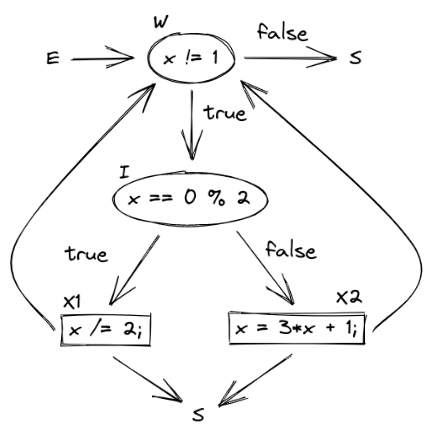
\includegraphics[scale=.4]{draw/draw5.png}
            \end{center}
            
            \vspace{6pt}
            
            \begin{tabular}{|p{50pt}|ccccccccccc|}
                \hline
                Chemin
                & E
                & $\rightarrow$
                & W
                & $\rightarrow$
                & I
                & $\rightarrow$
                & X1
                & $\rightarrow$
                & W
                & $\rightarrow$
                & S
                \\
                \hline
                $x$
                & $x_0$
                & \vline
                & $-$
                & \vline
                & $-$
                & \vline
                & $x_0 / 2$
                & \vline
                & $-$
                &&
                \\
                
                \hline
                Condition de chemin
                & vrai
                & \vline
                & $x_0 \neq 1$
                & \vline
                & $\begin{cases} x_0 \neq 1 \\ x_0 \equiv 0\ [2] \end{cases}\!\!\!\!\!\!\!\!$
                & \vline
                & $-$
                & \vline
                & $\begin{cases} x_0 \neq 1 \\ x_0 \equiv 0\ [2] \\ x_0 / 2 = 1\end{cases}\!\!\!\!\!\!\!\!$
                & \vline
                & $-$
                \\
                \hline
            \end{tabular}
            
            \vspace{6pt}
            
            Le chemin est faisable avec l'entrée $x = 2$.
            
            \vspace{12pt}
            
            \begin{tabular}{|p{50pt}|ccccccccccc|}
                \hline
                Chemin
                & E
                & $\rightarrow$
                & W
                & $\rightarrow$
                & I
                & $\rightarrow$
                & X2
                & $\rightarrow$
                & W
                & $\rightarrow$
                & S
                \\
                \hline
                $x$
                & $x_0$
                & \vline
                & $-$
                & \vline
                & $-$
                & \vline
                & $3x_0 + 1$
                & \vline
                & $-$
                &&
                \\
                
                \hline
                Condition de chemin
                & vrai
                & \vline
                & $x_0 \neq 1$
                & \vline
                & $\begin{cases} x_0 \neq 1 \\ x_0 \equiv 1\ [2] \end{cases}\!\!\!\!\!\!\!\!$
                & \vline
                & $-$
                & \vline
                & $\begin{cases} x_0 \neq 1 \\ x_0 \equiv 1\ [2] \\ 3x_0 + 1 = 1 \end{cases}\!\!\!\!\!\!\!\!$
                & \vline
                & $-$
                \\
                \hline
            \end{tabular}
            
            Le chemin est infaisable :
            $
                \begin{cases}
                    x_0 \equiv 1 \ [2]
                    \\
                    3x_0 + 1 = 1
                \end{cases}
            $
            : contradiction ($x_0$ impair donc $3x_0 + 1$ pair).
        \end{indt}
        
    \end{indt}

    
    
    
\end{document}
%--------------------------------------------End
